\section{Proposed Solution Description}

This section describes the high-level details of the proposed solution. 
It highlights the design principles, high-level architecture of the solution, data storage representation, operations, and also shows differences from the GraphBLAS API.

\subsection{Design Principles}

Spla library aims to address some of GraphBLAS standard limitations.
It is designed the way to maximize potential library performance, to simplify its implementation and extension, and to provide the end-user verbose, but expressive interface allowing customization and precise control over operations execution. 
These ideas are captured in the following principles.

\begin{itemize}
    \item \textit{Optional acceleration}. Library is designed in a way, that GPU acceleration is fully plugable and optional part. Library can perform computations using standard CPU pipeline. If GPU acceleration is presented, library can offload a part of a work for it. It allows both non-trivial processing of the data on the CPU only, as well as possibility to integrate different backends in the future.  
    \item \textit{User-defined functions}. The user can create custom element-wise functions to parameterize operations. Custom functions can be used for both CPU and GPU execution.
    \item \textit{Predefined scalar data types}. The library provides a set of built-in scalar data types that have a natural one-to-one relationship with native GPU built-in types. Data storage is transparent. The library interprets the data as POD-structures. The user can interpret individual elements as a sequence of bytes of a fixed size.
    \item \textit{Hybrid-storage format}. The library automates the process of data storage and preprocessing. It supports several data formats, chooses the best one depending on the situation.
    \item \textit{Exportable interface}. The library has a C++ interface with an automated reference-counting and with no-templates usage. It is compiled into a shared library. The interface is wrapped by C99 compatible API and exported to other languages, for example, in a form of a Python package.
    \item \textit{Introspection}. Each library class instantiates into a first-class object. Such objects can be captured, manipulated, passed as arguments and returned as function results. Parameterization types of containers can be inspected, as well as declared user functions.
\end{itemize}

\subsection{Architecture Overview}

The general idea of the proposed solution is depicted in Fig.~\ref{fig:design}. 
The core of the library and its main part is the CPU, which is the master node which controls all computations. 
It is responsible for storing data, maintaining a registry with algorithms, and scheduling operations to perform. 
In this paradigm, the GPU is an optional backend for acceleration, implemented through a special interface. 
It can optionally store data in a specific format. 
The CPU can offload the calculation of a part of the operations to the GPU, if the corresponding operation is supported by the given accelerator.

The reason for this is that the CPU and GPU are inherently asymmetric in nature. 
The end-user uses CPU side API. Thus, some preprocessing on the CPU side must be always done in the majority of cases. In addition, access to data on the GPU and their storage is carried out differently due to the peculiarities of the execution of kernels. 
Also, VRAM is more expensive and has less capacity than RAM.
Therefore, RAM is a cache for VRAM, and data duplication can be neglected. 
In the end, the explicit separation of the CPU side from the GPU backend gives the modularity. 
This can be used not only to support different GPU technologies, but also to integrate multiple GPUs or distributed processing in the future.

\begin{figure}[t]
\centering
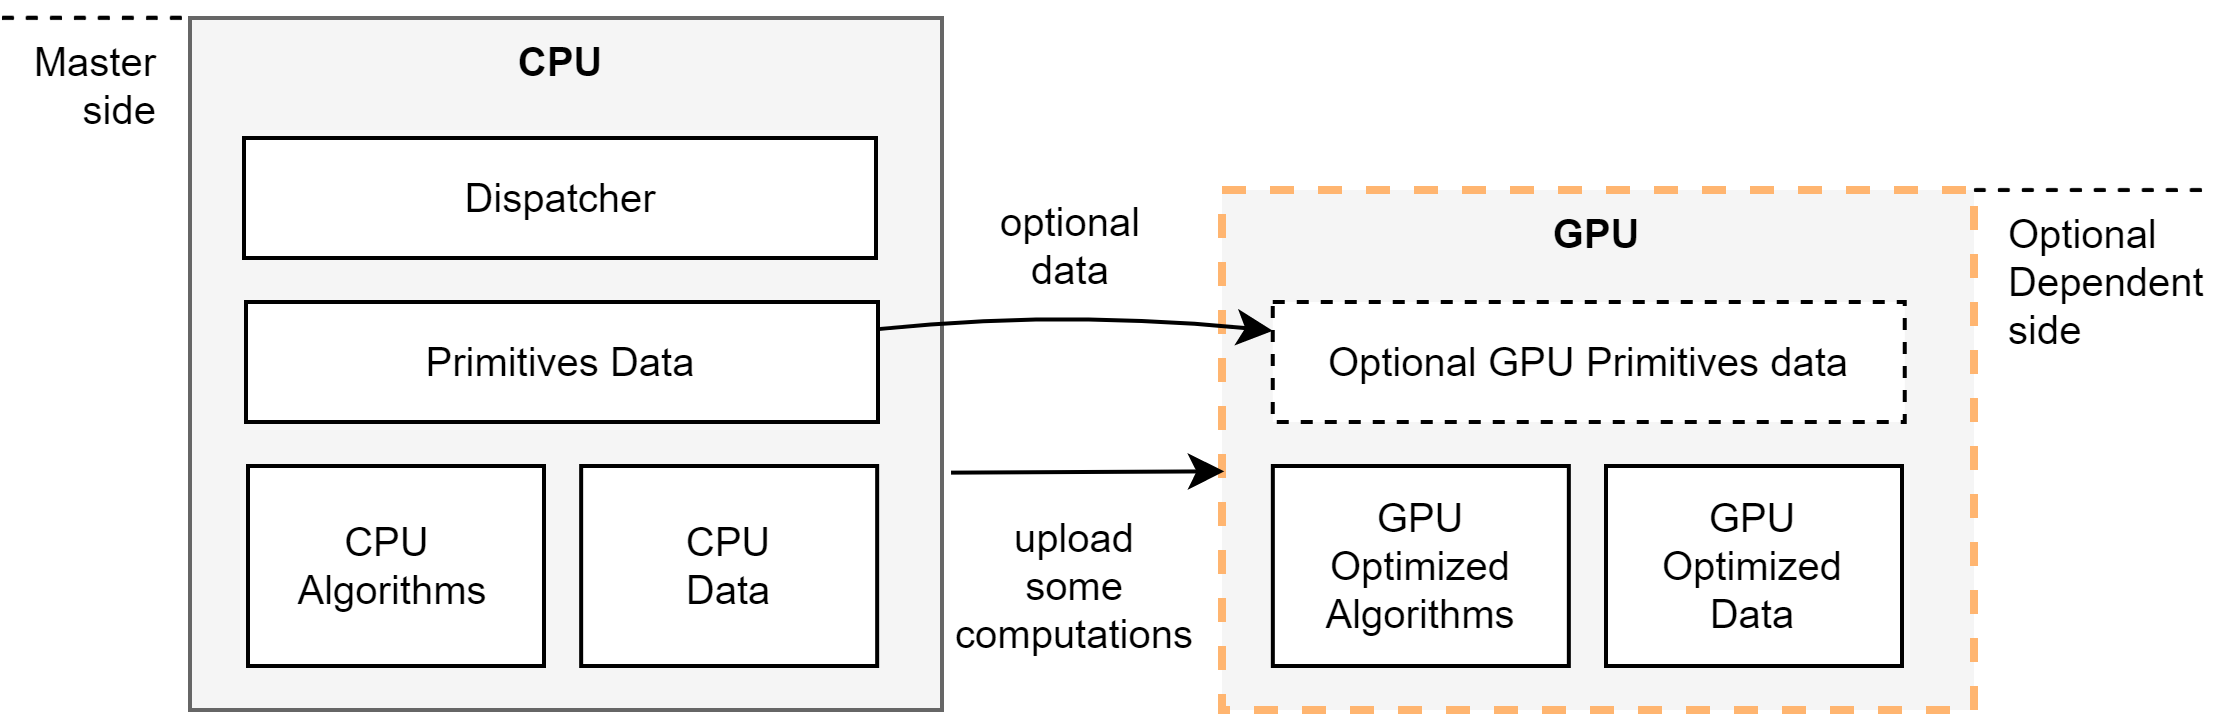
\includegraphics[width=0.95\linewidth]{figures/design_idea.png}
\caption{Proposed solution general design.}
\label{fig:design}
\end{figure}
    
\subsection{Data Containers}

Library provides general \textit{M-by-N Matrix}, \textit{N Vector}, \textit{Scalar} and \textit{N Array} data containers.
Underlying primitive value types are specified by \textit{Type} object. 
Single vector or matrix data is stored in specialized multi-format storage container. An example of the single vector storage is depicted in Fig.~\ref{fig:vec_storage}. 

The storage is responsible for keeping data in multiple different formats at the same time. 
Each format is best suited for a specific type of task and requested on demand. 
Key-value dictionary suites well frequent insertion, query or deletion operations, when memory usage and response time are critical. 
Mathematical operations perform better with compacted sequential lists of values since they have more friendly cache behaviour. 
GPU operations require separate format with a copy of the data resident in VRAM.

The storage and particular format can be inspected using array primitive. It allows one to get the view of an existing CPU or GPU buffer without actual copy, or initialize matrix or vector in particular format from existing arrays, which may be created and filled by user code. Also array gives an ability to acquire raw pointer to memory or GPU buffer handler, what can be used for interoperability and seamless integration into user data pipeline.

Data transformation from one format to another is carried out using a special rules graph. Example graph for a vector storage is shown in Fig.~\ref{fig:vec_tsf}. 
The directed edges in this graph indicate conversion rules. 
The graph must be the single strongly connected component. 
An example of the data transformation process is depicted in Fig.~\ref{fig:vec_exmp}. 
For a requested format the best path of convertation is obtained. Currently, the shortest one is used. 
Weight assignment to rules can potentially be used to prioritize convertations for some formats. 

Currently, several storage formats are supported. 
There is dictionary of keys for vector and matrix (DoK), list of coordinates (COO), dense vector, list of lists (LIL) and compressed sparse rows (CSR) matrix formats.  
Other formats, such as CSC, DCSR, ELL, etc., can be added to the library by the implementation of formats conversion and by the specialization of operations for a specific format. 

\begin{figure}[b]
\centering
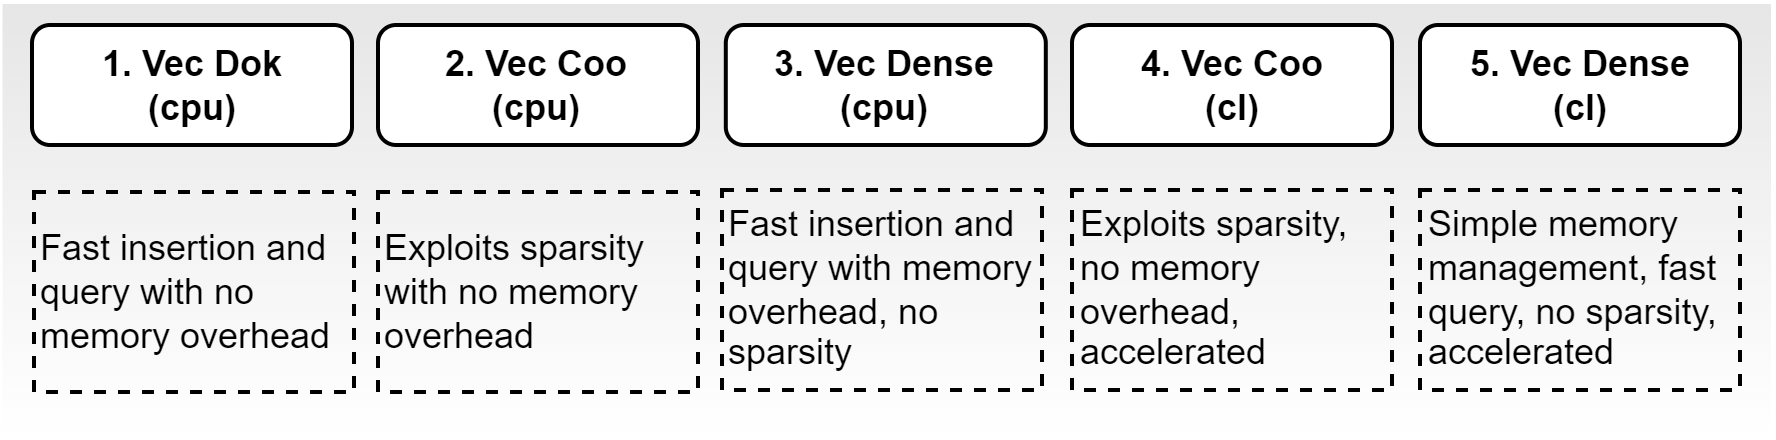
\includegraphics[width=0.8\linewidth]{figures/vector_storage.png}
\caption{Vector primitive storage holds the same data potentially in multiple different formats at the same time. Some slots can be empty.}
\label{fig:vec_storage}
\end{figure}

\begin{figure}[]
\centering
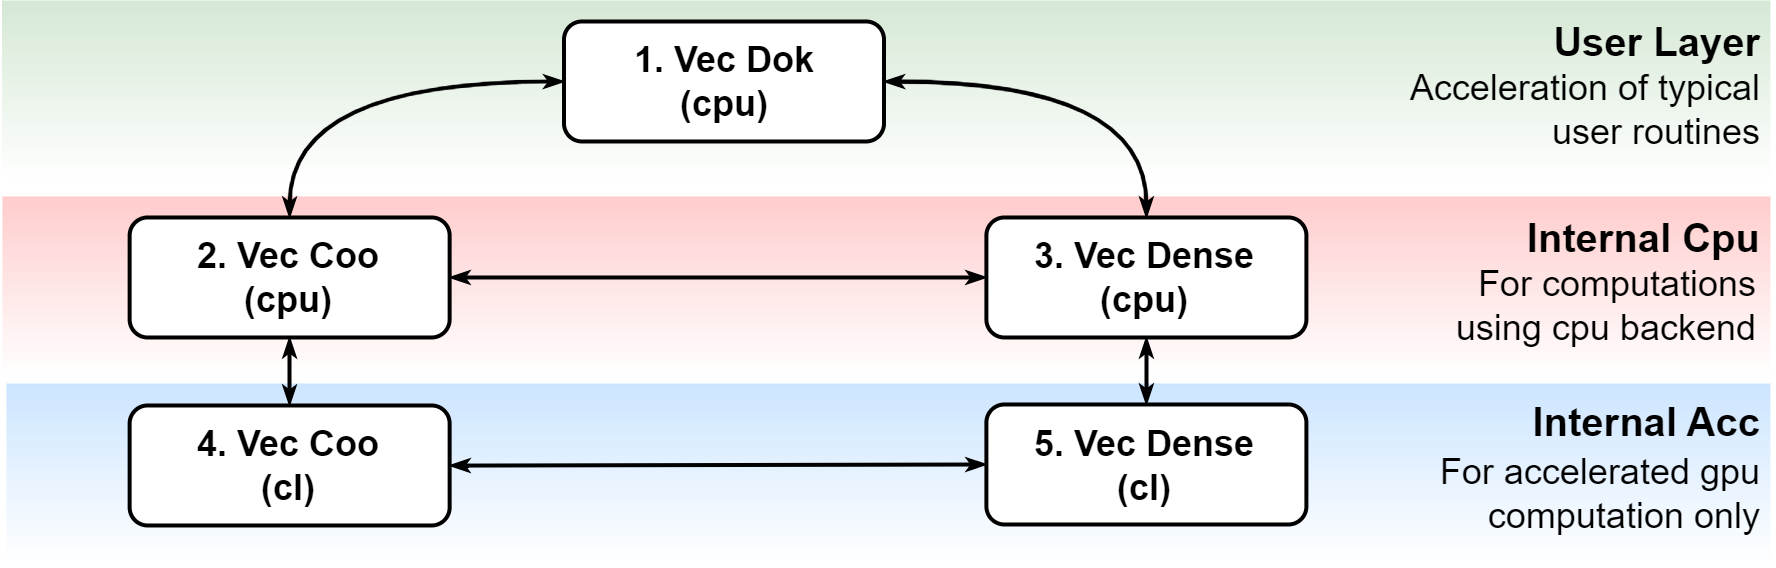
\includegraphics[width=0.8\linewidth]{figures/storage_transformation_graph.png}
\caption{Vector storage transformation graph. The graph defines how data can be obtained from one format in another.}
\label{fig:vec_tsf}
\end{figure}

\begin{figure}[]
\centering
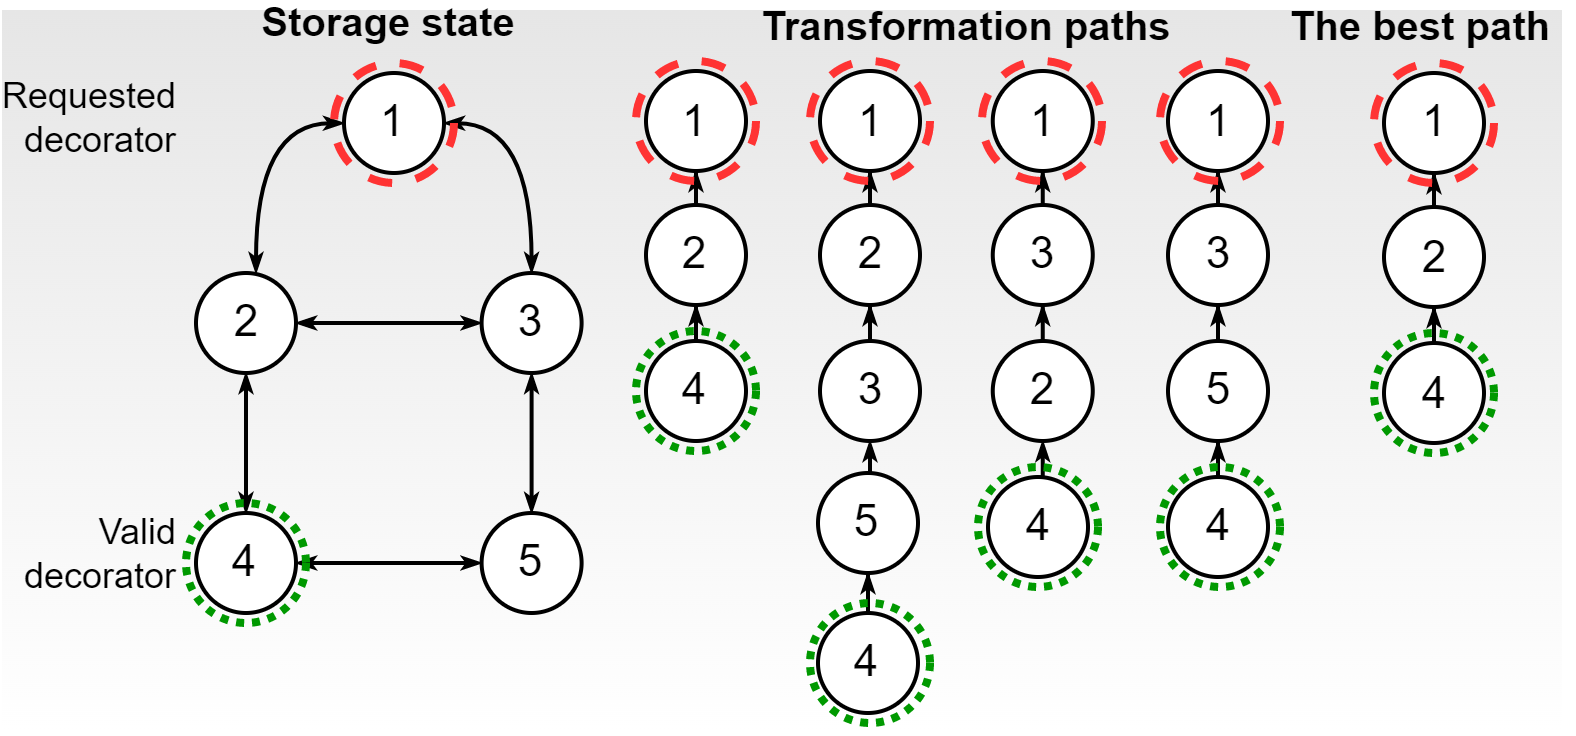
\includegraphics[width=0.8\linewidth]{figures/storage_transformation.png}
\caption{Vector storage transformation process. Green is valid format. Red is requested format. No highlight is currently invalid format.}
\label{fig:vec_exmp}
\end{figure}

\subsection{Algebraic Operations}

Library provides a number of commonly used operations, such as \textit{vxm}, \textit{mxv}, \textit{mxmT}, \textit{element-wise add}, \textit{assign}, \textit{map}, \textit{reduce}, etc.
Other operations can be added on demand.
Interface of operations is inspired by GraphBLAS standard. 
It supports \textit{masking}, parametrization by \textit{binary mult} and \textit{binary add} functions, \textit{select} for filtering and mask application, \textit{unary op} for values transformation, and \textit{descriptor} object for additional operation tweaking.

\subsection{Differences with GraphBLAS standard}

To be clear, the proposed solution is not an implementation of GraphBLAS C or C++ API. 
The design of the library uses only the concepts described by the standard. 
Thus, the signatures and semantics of some of the operations have been changed in the proposed solution. 
The API has been made more verbose and explicit. 
In particular, the handling of \textit{zero} elements and \textit{masking} are made cleaner for the end user. The library interprets data simply as collections of bytes, without mathematical semantics.
Identity element must be explicitly passed by the user where required. Mask applied using separate user-defined predicate for selection. Special fill value used for sparse-dense convertations. It allows to make the memory usage predictable and the result of each operation clear to the end user without internal implicit storage manipulations.